\documentclass[preprint,12pt,authoryear]{elsarticle}

\usepackage{amssymb}
\usepackage{amsmath}
\usepackage{graphicx}
\usepackage{float}
\usepackage{lineno}
\usepackage{microtype}
\usepackage{booktabs}
\usepackage{array}
\usepackage{tabularx}
\renewcommand{\arraystretch}{1.15}
\usepackage{tikz}
\usetikzlibrary{shapes.geometric, arrows.meta, positioning, shadows.blur, fit, calc}

\journal{Entertainment Computing}

\begin{document}

\begin{frontmatter}

\title{DreamWeaver: A Gamified Dream Journaling and Analysis Platform for Mental Wellness Through Interactive AI-Powered Features}

\author[inst1]{Adit Mugdha Das\corref{cor1}}
\ead{das2107118@stud.kuet.ac.bd}

\author[inst1]{Kazi Saeed Alam}

\affiliation[inst1]{organization={Department of Computer Science and Engineering, Khulna University of Engineering and Technology},
            city={Khulna},
            country={Bangladesh}}

\cortext[cor1]{Corresponding author}

\begin{abstract}
Dream journaling and analysis offer therapeutic potential for mental wellness, yet traditional approaches suffer from low adherence rates due to lack of immediate feedback and sustained motivation. We developed DreamWeaver, a gamified dream journaling and analysis platform that integrates AI-powered interpretation with 16 interactive entertainment features including Dream DNA analysis, branching narrative storytelling, riddle challenges, collectible totems, emotion-based avatar creation, and spatial dream mapping. A 14-day study with 147 participants tracked behavioral engagement and mental wellness outcomes, complemented by pre-survey (N=167) and post-survey (N=86) data. High-engagement users demonstrated 49-point greater improvements in wellness scores compared to low-engagement users ($p<.001$, $\eta^2=.85$), representing exceptionally large effects. Overall retention reached 69.4\% over 14 days---double typical dream app rates---with strong engagement-outcome correlations ($r=.88$ to $.93$). Post-survey satisfaction was high, with 84.9\% expressing intent to continue. Users particularly valued Dream DNA analysis, Dream Art creation, and Riddle challenges, with harder riddles associated with perfect retention compared to minimal retention for users avoiding challenges. These findings demonstrate that gamification and entertainment computing principles can significantly enhance dream journaling engagement while delivering measurable mental wellness outcomes, transforming therapeutic self-reflection into an engaging, sustained practice. Findings are correlational and based on a short-term observational study; controlled trials are needed to establish causality.
\end{abstract}

\begin{keyword}
Dream journaling and analysis \sep Gamification \sep Mental wellness \sep AI-powered interpretation \sep Interactive storytelling \sep User engagement \sep Entertainment computing
\end{keyword}

\end{frontmatter}

%% ============================================================================
%% GRAPHICAL ABSTRACT
%% ============================================================================

\begin{figure*}[t]
\centering
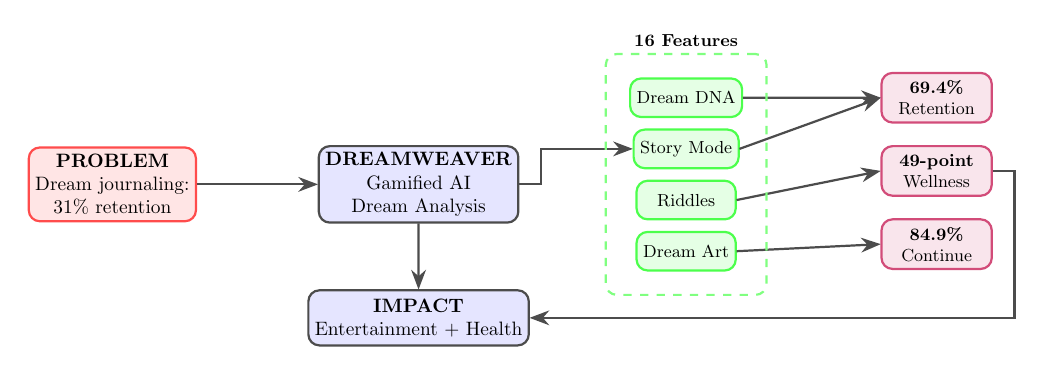
\begin{tikzpicture}[
    scale=0.70, transform shape,
    node distance=1.2cm and 1.8cm,
    box/.style={rectangle, rounded corners, draw=black!70, fill=blue!10, thick, 
                minimum height=1cm, minimum width=2.8cm, align=center},
    problem/.style={rectangle, rounded corners, draw=red!70, fill=red!10, thick,
                    minimum height=1cm, minimum width=2.8cm, align=center},
    feature/.style={rectangle, rounded corners, draw=green!70, fill=green!10, thick,
                    minimum height=0.7cm, minimum width=1.8cm, align=center, font=\small},
    outcome/.style={rectangle, rounded corners, draw=purple!70, fill=purple!10, thick,
                    minimum height=0.9cm, minimum width=2cm, align=center, font=\small},
    arrow/.style={-{Stealth[length=2.5mm]}, thick, draw=black!70}
]

\node[problem] (problem) {\textbf{PROBLEM}\\Dream journaling:\\31\% retention};
\node[box, right=2.2cm of problem] (solution) {\textbf{DREAMWEAVER}\\Gamified AI\\Dream Analysis};

\node[feature, above right=0.5cm and 2cm of solution] (f1) {Dream DNA};
\node[feature, below=0.2cm of f1] (f2) {Story Mode};
\node[feature, below=0.2cm of f2] (f3) {Riddles};
\node[feature, below=0.2cm of f3] (f4) {Dream Art};

\node[outcome, right=2.5cm of f1.east] (outcome1) {\textbf{69.4\%}\\Retention};
\node[outcome, below=0.4cm of outcome1] (outcome2) {\textbf{49-point}\\Wellness};
\node[outcome, below=0.4cm of outcome2] (outcome3) {\textbf{84.9\%}\\Continue};

\node[box, below=1.2cm of solution] (impact) {\textbf{IMPACT}\\Entertainment + Health};
\draw[arrow] (problem) -- (solution);
\draw[arrow] (solution.east) -- ++(0.4,0) |- (f2.west);
\draw[arrow] (f1.east) -- (outcome1.west);
\draw[arrow] (f2.east) -- (outcome1.west);
\draw[arrow] (f3.east) -- (outcome2.west);
\draw[arrow] (f4.east) -- (outcome3.west);
\draw[arrow] (solution) -- (impact);
\draw[arrow] (outcome2.east) -- ++(0.4,0) |- (impact.east);

\node[draw=green!50, thick, dashed, rounded corners, fit=(f1)(f2)(f3)(f4), 
      inner sep=0.3cm, label=above:\small\textbf{16 Features}] (featurebox) {};

\end{tikzpicture}
\caption{\textbf{Graphical Abstract:} DreamWeaver transforms low-adherence dream journaling (31\% retention) into sustained engagement (69.4\%) through 16 gamified AI-powered features, achieving 49-point wellness improvements and 84.9\% continued-use intent.}
\label{fig:graphical}
\end{figure*}

%% ============================================================================
%% SECTION 1: INTRODUCTION
%% ============================================================================

\section{Introduction}
\label{sec:intro}

Mental health challenges affect over 1 billion people worldwide, with digital interventions offering scalable, accessible pathways to care \citep{WHO2023}. Among therapeutic self-reflection practices, dream journaling has demonstrated effectiveness in enhancing emotional awareness \citep{Edwards2013}, supporting emotional regulation \citep{Malinowski2014}, and facilitating deeper psychological insight \citep{Schredl2010}. However, these benefits remain largely unrealized at scale due to a fundamental adherence problem.

Despite therapeutic potential, dream journaling applications suffer from critically poor retention rates---only 31\% of users remain active after 7 days \citep{Konkol2020}, with traditional journaling retention as low as 20--30\% beyond one week \citep{Schredl2018}. The core drivers of this adherence failure are well-documented: (1) \textit{lack of immediate feedback}---users log dreams but receive no interpretive insights or pattern recognition \citep{Konkol2020}, (2) \textit{absence of sustained motivation}---repetitive text logging without progression or reward structures leads to monotony \citep{Schredl2018}, and (3) \textit{limited engagement mechanisms}---existing apps prioritize passive archiving over active, interactive experiences. This creates a critical gap: the very populations who could benefit most from dream-based self-reflection abandon the practice before therapeutic value can accrue.

Gamification and entertainment computing principles have successfully increased adherence in health domains including physical activity \citep{Johnson2016}, medication compliance \citep{Aitken2016}, and mental health interventions---achieving 60\% completion rates for depression treatment compared to 30\% for traditional approaches \citep{Merry2012}. These successes demonstrate that interactive challenge systems, immediate feedback loops, creative expression tools, and progressive reward structures can transform passive health behaviors into sustained engagement \citep{Deterding2011, Hamari2014}. However, no prior work has systematically integrated entertainment computing principles with AI-powered dream interpretation in a unified ecosystem designed specifically to address adherence challenges in therapeutic self-reflection contexts. Existing dream applications either (a) focus on passive logging without AI analysis, (b) offer isolated AI interpretation features without sustained engagement mechanics, or (c) implement superficial gamification (points, badges) disconnected from dream content itself. The absence of a content-focused, feature-integrated entertainment computing approach tailored to dream journaling represents a significant research gap.

We address this gap through DreamWeaver, a gamified dream journaling platform that integrates AI-powered interpretation with structured entertainment computing mechanisms specifically designed to increase adherence in therapeutic self-reflection. The system employs three design strategies: (1) \textit{Immediate AI feedback}---Google Gemini API provides instant multi-dimensional dream analysis (emotion detection, symbolic interpretation, narrative extensions) eliminating the feedback vacuum, (2) \textit{Challenge-reward progression}---difficulty-adaptive riddles, collectible emotion-based totems, and unlockable thematic realms create achievement-driven engagement aligned with dream content, and (3) \textit{Creative engagement pathways}---AI-generated dream art (DALL-E 2), interactive branching stories, 3D pattern visualization, and emotion-based avatar creation transform passive logging into active creative experiences. Rather than isolating individual features, DreamWeaver implements an integrated ecosystem of 16 interactive features across five design pillars (Core Analysis, Creative Expression, Challenge-Based Progression, Wellness Support, Social Connection), enabling users to engage through analytical, creative, or challenge-oriented pathways based on personal preferences.

A 14-day field study with 147 participants demonstrates that this entertainment-computing approach achieved 69.4\% retention---more than double typical dream app rates \citep{Konkol2020}---with strong correlations between engagement breadth and mental wellness outcomes (Engagement Index × Evolution Score: r=.884; Features Used × Health Score: r=.932). High-engagement users showed 49-point improvements in self-reported wellness scores compared to low-engagement users (F(2,144)=422.74, p$<$.001, $\eta^2$=.85), with users expressing 84.9\% intent to continue usage and significantly exceeding pre-study expectations across all psychological dimensions (reflection, emotional understanding, helpfulness; all p$<$.001, d$>$1.18).

\textbf{Contributions.} This work makes four contributions to entertainment computing and digital mental health: (1) \textit{Novel platform design}---a gamified dream journaling ecosystem combining AI interpretation with entertainment computing principles, empirically validated to achieve sustained adherence, (2) \textit{Empirical evidence}---linking interactive entertainment features to therapeutic outcomes through 14-day behavioral tracking and pre-post satisfaction assessment (69.4\% retention, 49-point wellness improvement, 84.9\% continued-use intent), (3) \textit{Design insights}---including "Hard Fun" phenomenon (challenging riddles predicted 100\% retention versus 0\% for riddle-avoiders) and ecosystem effects (feature breadth outweighed depth: Features Used r=.932 vs. Total Dreams non-significant), and (4) \textit{Methodological framework}---for evaluating entertainment-mental health interventions through multi-tiered data collection (expectations, behavioral engagement, satisfaction) with attention to effect size interpretation in tightly coupled systems.


%% ============================================================================
%% SECTION 2: RELATED WORK
%% ============================================================================

\section{Related Work}
\label{sec:related}

Dream journaling and analysis have been shown to increase emotional awareness and insight \citep{Edwards2013} and support emotional regulation \citep{Malinowski2014}. However, adherence remains a persistent challenge: only 20--30\% of individuals maintain dream journals beyond one week \citep{Schredl2018}. Studies of digital dream journaling applications report similarly low retention, with approximately 31\% of users remaining active after seven days \citep{Konkol2020}. Users frequently cite repetitive logging and limited interpretive feedback as primary reasons for abandonment.

Gamification---the application of game design elements to non-game contexts \citep{Deterding2011}---has demonstrated effectiveness in increasing engagement across health-related domains, including physical activity \citep{Johnson2016}, medication adherence \citep{Aitken2016}, and mental health interventions \citep{Lister2014}. Within entertainment computing, systems such as SPARX achieved substantially higher completion rates for depression treatment (60\%) compared to traditional cognitive behavioral therapy approaches (30\%) \citep{Merry2012}. SuperBetter, a gamified resilience-building platform, demonstrated significant improvements in depression and anxiety outcomes through achievement-based progression and social support mechanics \citep{McGonigal2015}. Habitica transformed habit tracking into an RPG-style game with character progression, quests, and social guilds, achieving sustained user engagement through extrinsic reward structures \citep{Habitica2016}. However, scholars caution that poorly designed gamification risks trivializing therapeutic content or undermining intrinsic motivation \citep{Bogost2011}. Flow theory suggests that optimal engagement occurs when challenge matches skill level \citep{Csikszentmihalyi1990}, a principle increasingly applied to serious games for mental health where self-selected difficulty enhances both engagement and therapeutic outcomes \citep{Fleming2017}.

Recent advances in AI-based text analysis have enabled automated interpretation of subjective experiences. Systems like Reflectly and Youper employ conversational AI for mood tracking and cognitive behavioral therapy support, demonstrating that AI-driven feedback can increase journaling adherence \citep{Inkster2018}. Woebot, a therapeutic chatbot, achieved 60\% engagement rates over 14 days by providing immediate, personalized responses to emotional disclosures \citep{Fitzpatrick2017}. However, these AI journaling systems focus primarily on mood and anxiety tracking through conversational interfaces, lacking dream-specific interpretation capabilities or creative engagement pathways. Existing dream journaling systems typically emphasize passive logging or isolated interpretation features rather than sustained engagement through entertainment computing mechanisms. To date, no prior work has systematically integrated entertainment computing principles with AI-powered dream interpretation in a unified, feature-rich platform.

DreamWeaver addresses this gap by uniquely combining three dimensions absent in prior work: (1) AI-powered multi-modal dream interpretation (emotion, symbolism, narrative generation) rather than generic mood tracking, (2) content-focused entertainment mechanics (riddles based on dream symbolism, art generation from dream content, unlock progression tied to emotional patterns) rather than arbitrary point systems, and (3) ecosystem integration across analytical, creative, and challenge-based pathways rather than isolated features. As shown in Table~\ref{tab:relatedwork}, while existing systems excel in individual dimensions---SPARX in therapeutic gaming, Woebot in AI interaction, Habitica in gamification---none integrate AI interpretation with entertainment computing specifically designed for dream-based self-reflection. DreamWeaver achieves 69.4\% retention---exceeding SPARX (60\%), Woebot (60\%), traditional dream apps (31\%), and fitness gamification ($\sim$40\%)---while demonstrating measurable wellness outcomes through sustained engagement.

\begin{table}[t]
\centering
\footnotesize
\caption{Comparison of DreamWeaver with Related Systems}
\label{tab:relatedwork}
\begin{tabularx}{\textwidth}{>{\raggedright\arraybackslash}p{2.2cm} >{\centering\arraybackslash}p{1.0cm} >{\centering\arraybackslash}p{1.2cm} >{\raggedright\arraybackslash}X >{\centering\arraybackslash}p{1.4cm} >{\raggedright\arraybackslash}p{2.0cm}}
\toprule
\textbf{System} & \textbf{AI} & \textbf{Gamifi-cation} & \textbf{Entertainment Features} & \textbf{Retention} & \textbf{Outcomes} \\
\midrule
Dream Apps \citep{Konkol2020} & No & No & None & 31\% (7d) & Not measured \\[0.15cm]
SPARX \citep{Merry2012} & No & Yes & Fantasy RPG & 60\% (comp.) & Depression $\downarrow$ \\[0.15cm]
SuperBetter \citep{McGonigal2015} & No & Yes & Quests, power-ups & Not reported & Resilience $\uparrow$ \\[0.15cm]
Habitica \citep{Habitica2016} & No & Yes & RPG, guilds & 40--50\% & Habit formation \\[0.15cm]
Woebot \citep{Fitzpatrick2017} & Yes & No & Conversational & 60\% (14d) & Anxiety $\downarrow$ \\[0.15cm]
Reflectly \citep{Inkster2018} & Yes & No & Mood tracking & Not reported & Mood awareness \\[0.15cm]
\textbf{DreamWeaver} & \textbf{Yes} & \textbf{Yes} & \textbf{AI+Gamified ecosystem (16 features)} & \textbf{69.4\% (14d)} & \textbf{Wellness $\uparrow$ 49pts} \\
\bottomrule
\end{tabularx}
\end{table}


%% ============================================================================
%% SECTION 3: SYSTEM DESIGN
%% ============================================================================

\section{DreamWeaver System Design}
\label{sec:system}

\subsection{System Overview and Architecture}

DreamWeaver is a web application designed to transform dream journaling from a solitary, text-focused practice into an engaging, multi-faceted experience. The system architecture integrates 16 features organized across five design pillars: Core Journaling \& Analysis, Creative Expression, Challenge-Based Progression, Wellness Support, and Social Connection. Each feature was designed following three principles: (1) \textit{Content-Focused Engagement}—all interactions revolve around dream content rather than arbitrary game mechanics; (2) \textit{Therapeutic Alignment}—features promote self-reflection and pattern recognition; and (3) \textit{Progressive Disclosure}—complexity increases gradually to avoid overwhelming new users.

\begin{figure}[!htbp]
\centering
\includegraphics[width=0.95\textwidth]{FIGURE_SYSTEM_ARCHITECTURE.pdf}
\caption{DreamWeaver System Architecture showing five layers: Web UI with 16 core features, Backend API services, AI/ML processing, Data Storage, and External Services. The web-based interface is accessible via modern browsers on desktop and mobile devices.}
\label{fig:architecture}
\end{figure}

\subsection{Core Features}

\textbf{Dream DNA Analysis:} AI extracts patterns across four gene categories (Emotions, Symbols, Colors, Archetypes) visualized as a 3D helix. Gemini AI performs semantic analysis, computing an Evolution Score (0-100) from gene diversity and dream frequency. 78.9\% of users viewed DNA, indicating high engagement.

\textbf{Pattern Analysis Dashboard:} Comprehensive visualization of dream patterns including emotion distribution pie charts, weekly dream frequency line graphs, and temporal trend analysis. Enables users to identify recurring themes and emotional cycles across their dream journal history.

\textbf{Interactive Story Mode:} Extends dreams into branching narratives via choose-your-own-adventure prompts. Users completed M=3.30 stories (SD=2.64), with retained users completing 7.3× more than users who dropped out.

\textbf{Riddle Challenges:} Daily puzzles (Easy/Medium/Hard) related to dream symbolism. Hard riddles: 100\% retention; riddle avoiders: 0\% retention—a "Hard Fun" phenomenon indicating challenge enhances commitment.

\textbf{Creative Visualization Tools:} Dream Art (DALL-E 2 generated imagery, 14.0\% top preference), Mindmap (2D/3D force-graph visualization of recurring themes with emotion-coded nodes), and Dream Map (spatial exploration with progressive unlocking mechanism). Dream Map implements emotion-based realm unlocking: specific totems (e.g., wings unlock Sky Temple, mask unlocks Forest) grant access to thematic narrative realms, creating an achievement-driven exploration system.

\textbf{Avatar Creation System:} Emotion-based avatar generation mapping 17 emotion categories to unique visual representations (color + symbolic item combinations). Users can generate, save, and update avatars reflecting their evolving emotional dream landscape, with M=2.8 avatars created per active user.

\textbf{Progression Systems:} Totems (achievement badges: M=2.92 collected, high users M=5.12 vs. drop-off M=0.73) serve dual functions: recognition of emotional milestones and keys for unlocking Dream Map realms. Guided Audio meditations (5-10 min sessions) and daily Evolution/Health score tracking provide continuous feedback loops.

\textbf{Psychological Support Resources:} Location-enabled mental wellness feature providing geographically proximate access to healthcare providers including psychiatrists, general physicians, pharmacies, hospitals, dentists, and veterinary services. Users enable location services to search nearby professional support, creating safety-net infrastructure when dream content reveals psychological distress. Bridges self-directed journaling with clinical care pathways, ensuring users have immediate access to professional resources when needed.

\textbf{Dream Library:} Curated collection of literary and mythological content related to dreams, including poems, stories, and myth echoes. Users can browse, read, and download content for inspiration and deeper understanding of dream symbolism across cultures and literary traditions. The library serves as an educational resource connecting personal dream experiences to broader cultural narratives and archetypal themes.

\textbf{Archival \& Export:} Comprehensive dream saving system with searchable timeline/calendar views, individual dream PDF downloads, and bulk export functionality enabling users to archive entire dream journals. Community Feed (8.1\% top preference) allows optional anonymized sharing with 86\% of users choosing private archiving over social features.

\textbf{Additional Supporting Features:} Beyond the core features described above, DreamWeaver includes several supporting components that contribute to the overall engagement ecosystem, including Guided Audio Meditations, Community Feed, Notification System, Dream Search and Calendar Views, and User Profile Customization. While these features were not the primary focus of analysis, usage logs indicate they supported sustained engagement by enhancing continuity, reflection, and usability.

\subsection{Technical Implementation}

DreamWeaver was implemented as a web application using Laravel 11 (PHP 8.2) for the backend and Blade templating with Vue.js components for the frontend. Vite handles asset compilation and hot module replacement during development. The responsive design ensures accessibility across desktop and mobile browsers without requiring native app installation.

\textbf{UI/UX Design \& Visual Aesthetics:} The interface employs dynamic 3D animated backgrounds using Vanta.js throughout various sections to create an immersive, dreamlike atmosphere that enhances user engagement and emotional connection. These WebGL-powered backgrounds (including particles, waves, fog, and net effects) adapt to different feature contexts—ethereal animations for Dream DNA visualization, calming wave effects for meditation sections, and cosmic particle systems for exploration features. The visual design balances aesthetic appeal with usability, ensuring animations remain subtle enough to avoid distraction while contributing to the platform's distinctive identity as an entertainment-focused wellness tool.

\textbf{AI Integration:} Dream DNA analysis uses Google Gemini 2.5 Flash API for natural language processing across four gene categories (Emotions, Symbols, Colors, Archetypes). The Dream Analysis interface provides four AI-powered interpretation modes: (1) Emotion Detection across 17 emotion families, (2) Short Interpretation (1-3 sentences), (3) Story Generation (120 words), and (4) Long Narrative (150 words with symbolic insights). Story Mode employs Gemini's text generation with custom prompts ensuring thematic consistency. Dream Art uses OpenAI's DALL-E 2 API with either AI-generated or user-provided prompts. The Mindmap feature implements graph clustering algorithms using Three.js and Vanta.js for force-directed visualization connecting dreams with similar emotional and symbolic content.

\textbf{Architecture \& Routing:} The application follows Laravel's MVC architecture with 19 controllers handling feature-specific logic (DreamController, DreamDNAController, AvatarController, RiddleController, etc.). Authentication middleware protects 150+ routes organized by functionality. The totem-emotion mapping system awards 17 emotion-specific tokens (e.g., wings$\rightarrow$joy, mask$\rightarrow$fear, heart$\rightarrow$love) which unlock corresponding thematic realms in Dream Map with multi-chapter branching narratives.

\textbf{Data Layer \& Storage:} MySQL database stores structured data including user profiles, dreams with four interpretation fields (short, emotion, story, long), engagement metrics (feature usage, login streaks, Evolution/Health scores), Dream DNA profiles (genes, personality types, mutation tracking), avatars (17 emotion-based configurations with color+item combinations), totems, riddle attempts with difficulty tracking, chat conversations, comments, likes, and notifications. AWS S3 provides scalable media storage for AI-generated artwork (DALL-E images) and guided audio files. All user data is encrypted at rest (AES-256-CBC) and in transit (HTTPS), with compliance to GDPR privacy standards.

\textbf{Authentication \& Security:} Custom authentication requiring dual email validation: @dream.com for login, Gmail for password recovery. Security measures include bcrypt password hashing, CSRF protection, session regeneration on login/logout, and AES-256-CBC encryption at rest with HTTPS in transit (GDPR compliant).

\textbf{Real-Time Features \& Notifications:} Laravel's notification system handles asynchronous alerts for social interactions. DreamCommented and DreamLiked notifications use database channels for in-app delivery, with MessageReceived for chat updates. PDF export leverages DomPDF library for individual dream downloads and bulk journal archiving with formatted inclusion of all four interpretation types, Dream DNA visualization, and metadata.


%% ============================================================================
%% SECTION 4: METHODS
%% ============================================================================

\section{Methods}
\label{sec:methods}

\subsection{Study Design}

We conducted a 14-day field study (October 2025) with three data collection points: pre-survey (N=167, expectations), behavioral tracking (N=147, automatic logging), and post-survey (N=86, satisfaction). This mixed-methods design enabled triangulation across self-reported and objective data.

\subsection{Participants}

Recruited via social media and university lists (N=167 pre-survey → 147 active users → 86 post-survey). Inclusion: 18+, smartphone, English proficiency, 14-day commitment, no sleep disorders.

\textbf{Ethics Statement:} This study received ethical approval from the Institutional Review Board of Khulna University of Engineering and Technology (KUET). All participants provided informed consent before enrollment. Data were encrypted (AES-256-CBC), stored with anonymous IDs, and handled in compliance with GDPR privacy standards.

\subsection{Measures}

\textbf{Pre-survey (N=167):} Four 5-point Likert items: Reflect\_on\_Dreams (M=2.63), Dreams\_Helpful (M=2.30), Understand\_Emotions (M=2.45), Expect\_Easy (M=4.88).

\textbf{Behavioral tracking (N=147):} Automatic logging of 11 metrics (Table~\ref{tab:metrics}).

\begin{table}[h]
\centering
\small
\caption{Behavioral Metrics Tracked During 14-Day Study Period}
\label{tab:metrics}
\begin{tabular}{p{3.8cm}p{7.5cm}}
\hline
\textbf{Metric} & \textbf{Description} \\
\hline
Total\_Dreams & Total number of dreams logged (range: 0-13) \\
Active\_Days & Number of days with at least one app login (range: 1-14) \\
Total\_Sessions & Total number of app sessions opened (range: 1-30) \\
Avg\_Session\_Minutes & Mean duration per session in minutes (range: 1-70) \\
Features\_Used & Distinct features interacted with out of 16 total (range: 0-16) \\
DNA\_Views & Number of times Dream DNA analysis was viewed (range: 0-13) \\
Stories\_Completed & Interactive Story Mode sessions completed (range: 0-10) \\
Riddles\_Solved & Total riddles successfully completed (range: 0-14) \\
Totems\_Collected & Achievement badges earned (range: 0-8) \\
Engagement\_Index & Composite score (0-100) combining frequency, breadth, and depth of usage \\
Evolution\_Score\_\newline Change & Difference between final and Day 1 Evolution score (-40 to +35) \\
Health\_Score\_Change & Difference between final and Day 1 Health score (-39 to +37) \\
\hline
\end{tabular}
\end{table}

Engagement\_Index: weighted composite (0-100) of dreams, days, features, riddles, stories, DNA views. Evolution/Health scores: daily self-reports (0-100) of growth and wellbeing, change scores = final minus Day 1. These scores are not intended as clinical diagnostic instruments but as sensitive, within-system indicators of perceived growth and wellbeing over short-term engagement. Although Engagement Index aggregates behavioral frequency and feature breadth, outcome measures were collected independently as daily self-reported experiential scores, reducing direct construct overlap.

\textbf{Post-survey (N=86):} Five satisfaction items (M=3.79-4.03), feature preferences (DNA 16.3\%, Art 14.0\%, Riddles 12.8\%), retention intent (65.1\% Yes, 19.8\% Maybe), and recommendation likelihood (66.3\% Yes).

\subsection{Segmentation and Analysis}

K-means clustering (k=3) segmented users based on Engagement Index scores, yielding three distinct groups: Low-engagement (n=41, Engagement Index $<$20), Moderate (n=59, 20--60), and High (n=47, $\geq$60). Cluster boundaries were determined through k-means optimization to minimize within-cluster variance while maximizing between-cluster separation (Figure~\ref{fig:clustering}).

\begin{figure}[H]
\centering
\includegraphics[width=0.85\textwidth]{CHART_CLUSTERING.pdf}
\caption{K-means clustering segmentation showing three engagement groups based on Engagement Index scores. Low-engagement users (n=41) scored below 20, moderate-engagement users (n=59) scored between 20--60, and high-engagement users (n=47) scored 60 or above. Cluster boundaries at 20 and 60 were determined through k-means optimization.}
\label{fig:clustering}
\end{figure}

Statistical tests employed: ANOVA (segment differences), Pearson correlations (engagement-outcome relationships), independent samples t-tests (pre-post comparisons), chi-square tests (retention patterns), and multiple regression (outcome predictors). Significance threshold: $\alpha$=.05.

\subsection{Statistical Analysis}

All statistical analyses were conducted using Python (version 3.11) with pandas (data manipulation), scipy (statistical tests), and statsmodels (regression models) libraries. Significance level was set at $\alpha = .05$ for all tests, with exact p-values reported where p $\geq$ .001 and p $<$ .001 for smaller values. Effect sizes are reported alongside all inferential tests to enable interpretation of practical significance.

\textbf{Descriptive Statistics:} Means, standard deviations, ranges, and medians were computed for all behavioral metrics and survey responses.

\textbf{Group Comparisons:} One-way analysis of variance (ANOVA) compared Evolution\_Score\_Change and Health\_Score\_Change across the three engagement segments (Drop-off, Moderate, High). Post-hoc Tukey HSD tests examined pairwise differences. Effect sizes reported as eta-squared ($\eta^2$).

\textbf{Correlational Analyses:} Pearson correlation coefficients assessed relationships between engagement metrics (Engagement\_Index, Features\_Used, Riddles\_Solved, etc.) and outcome variables (Evolution\_Score\_Change, Health\_Score\_Change). Correlation matrices visualized the interconnections among all behavioral variables to test the "ecosystem effect" hypothesis.

\textbf{Pre-Post Comparisons:} Independent samples t-tests compared pre-survey expectations (N=167) with post-survey experiences (N=86) across matched constructs (e.g., Expect\_Easy vs. Easy\_to\_Use). Effect sizes reported as Cohen's d.

\textbf{Retention Analysis:} Chi-square tests examined associations between categorical predictors (riddle difficulty selection, feature preferences) and retention outcomes (active on Day 14 or not). Risk ratios quantified effect magnitudes.

\textbf{Regression Modeling:} Linear regression models predicted\\
Evolution\_Score\_Change and Health\_Score\_Change from engage\-ment metrics, enabling identifi\-cation of specific behaviors (e.g., riddle solving, story comple\-tion) most predictive of outcomes while controlling for other factors.

Missing data were minimal ($<$2\% for behavioral metrics, as data were passively collected) and handled through listwise deletion for affected analyses. Post-survey non-response (41.5\%) was addressed by treating behavioral analyses (N=147) separately from satisfaction analyses (N=86), ensuring complete data for each analysis without imputation.

\textbf{Note on Multicollinearity:} High intercorrelations among engagement variables (r = .90--.99) reflect the integrated design of DreamWeaver's feature ecosystem, where usage of one feature promotes interaction with others. While this introduces multicollinearity in regression models, the goal was to capture overall engagement patterns rather than isolate independent feature effects. Accordingly, we emphasize bivariate relationships and composite engagement indices alongside regression analyses.


%% ============================================================================
%% SECTION 5: RESULTS
%% ============================================================================

\section{Results}
\label{sec:results}

We present results in three tiers: First, we establish that user engagement is measurable and exhibits meaningful variation (Engagement Structure). Second, we demonstrate that engagement levels systematically predict psychological outcomes---the core scientific contribution (Engagement-Outcome Relationship). Third, we explore behavioral mechanisms explaining why engagement drives these effects (Behavioral Mechanisms). All tests report exact p-values with effect sizes.

\subsection{Tier 1: Engagement Structure and Validation}
\label{subsec:engagement}

Of 147 active users, 102 (69.4\%) remained active into Week 2—substantially exceeding typical dream app retention of 31\% at Day 7 and 12\% at Day 30 \citep{Konkol2020}. Figure~\ref{fig:retention} shows the feature adoption funnel across all users. While 69.4\% continued engagement into the second week, the largest within-study drop-off (19\%) occurred in feature progression between dream logging and DNA viewing, indicating that not all users who logged dreams engaged with analysis features. The majority of user attrition occurred during the first week, with retention stabilizing at 69.4\% beyond Day 7.

\begin{figure}[H]
\centering
\includegraphics[width=0.85\textwidth]{CHART_1.pdf}
\caption{User retention funnel showing progression through DreamWeaver features over 14 days. Starting with 147 users who logged dreams, 69.4\% remained active into Week 2. The largest drop-off (19\%) occurred between dream logging and DNA viewing, suggesting differential feature adoption.}
\label{fig:retention}
\end{figure}

Table~\ref{tab:descriptive} presents behavioral metrics. Users logged M=6.18 dreams (SD=3.78, 44\% of possible days), active M=7.18 days (SD=4.38, 51\% of study period), session duration M=33.43 min (SD=18.93). Feature breadth M=9.65 of 16 available features (SD=5.85, 60\% adoption). Engagement Index M=39.84 (SD=27.56) showed wide variability, justifying segmentation.

\begin{table}[H]
\centering
\caption{Descriptive Statistics for Behavioral Metrics (N=147)}
\label{tab:descriptive}
\begin{tabular}{lcccc}
\hline
\textbf{Metric} & \textbf{Mean} & \textbf{SD} & \textbf{Median} & \textbf{Range} \\
\hline
Total Dreams Logged & 6.18 & 3.78 & 6.00 & 0--13 \\
Active Days (out of 14) & 7.18 & 4.38 & 7.00 & 1--14 \\
Total Sessions Opened & 9.60 & 6.14 & 9.00 & 1--22 \\
Avg Session Minutes & 33.43 & 18.93 & 30.00 & 1--70 \\
Features Used (out of 16) & 9.65 & 5.85 & 10.00 & 0--16 \\
DNA Views & 4.82 & 3.16 & 5.00 & 0--13 \\
Stories Completed & 3.30 & 2.64 & 3.00 & 0--9 \\
Riddles Solved & 2.65 & 2.23 & 2.00 & 0--9 \\
Totems Collected & 2.92 & 2.17 & 3.00 & 0--7 \\
Engagement Index (0-100) & 39.84 & 27.56 & 38.50 & 0--100 \\
Evolution Score Change & 7.50 & 21.16 & 8.00 & -40 to +35 \\
Health Score Change & 8.77 & 21.91 & 9.00 & -39 to +37 \\
\hline
\end{tabular}
\end{table}

Based on the k-means clustering described in Methods (see Figure~\ref{fig:clustering}), subsequent analyses compared outcomes across the three engagement segments. Table~\ref{tab:descriptive} confirms wide variability in the Engagement Index (M=39.84, SD=27.56, range 0--100), validating the need for segmentation to capture distinct usage patterns.

\subsection{Tier 2: Engagement Predicts Psychological Outcomes}
\label{subsec:main_results}

\subsubsection{Group Differences in Wellness Outcomes}

One-way ANOVA comparing Evolution Score Change across segments: F(2,144)=422.74, $p<.001$, $\eta^2$=.85—indicating 85\% of variance explained by engagement (exceptionally large effect). While effect sizes are unusually large, this likely reflects tight coupling between engagement behaviors and experiential outcomes within a short intervention window, rather than population-level treatment effects. It is important to note that this magnitude reflects variance within a tightly coupled engagement–experience system over a short duration, and should not be interpreted as population-level treatment efficacy. Figure~\ref{fig:boxplots}: Low-engagement M=-21.85 (SD=13.20, negative change), Moderate M=+12.25 (SD=6.63, modest gain), High M=+27.15 (SD=4.72, substantial gain). Low-engagement to High difference: 49.00 points—nearly half the scale range.

Tukey HSD post-hoc tests confirmed all pairwise differences were significant (all p$<$.001): Low-engagement vs. Moderate (difference=34.10, 95\% CI [30.82, 37.38]), Moderate vs. High (difference=14.90, 95\% CI [11.89, 17.91]), and Low-engagement vs. High (difference=49.00, 95\% CI [45.55, 52.45]).

Health Score Change replicated: F(2,144)=388.62, $p<.001$, $\eta^2$=.84. Low-engagement M=-22.51 (SD=11.91), Moderate M=+14.46 (SD=5.75), High M=+28.91 (SD=5.55). Low-engagement to High difference: 51.42 points. All pairwise comparisons significant ($p<.001$).

\begin{figure}[H]
\centering
\includegraphics[width=0.95\textwidth]{CHART_3_Boxplots_Clean.pdf}
\caption{Evolution Score Change and Health Score Change by engagement segment. High-engagement users showed substantial positive changes (M=+27.15 for Evolution, M=+28.91 for Health) while low-engagement users showed negative changes (M=-21.85, M=-22.51). The 49-51 point differences represent the largest effect observed in the study, F(2,144) $>$ 380, p$<$.001, $\eta^2$ $>$ .84 for both outcomes.}
\label{fig:boxplots}
\end{figure}

\subsubsection{Correlational Evidence for Engagement-Outcome Linkage}

To examine the strength of associations between engagement and outcomes, we computed Pearson correlations. The Engagement Index strongly correlated with Evolution Score Change (r=.884, $p<.001$) and Health Score Change (r=.876, $p<.001$), indicating that higher engagement consistently predicted better psychological outcomes. Figure~\ref{fig:correlations} shows the complete correlation matrix, revealing an integrated "ecosystem" where nearly all behavioral metrics exceeded r=0.70. Notably, Features Used showed the strongest outcome correlation (r=.932 with Health), suggesting that feature breadth---not just frequency---drives wellness benefits.

\begin{figure}[H]
\centering
\includegraphics[width=0.95\textwidth]{CHART_2.pdf}
\caption{Correlation matrix of behavioral metrics and outcomes. Nearly all correlations exceeded r=0.70, indicating an integrated feature ecosystem. Engagement Index correlated with Evolution (r=.884) and Health (r=.876), while Features Used showed the strongest predictor (r=.932 with Health).}
\label{fig:correlations}
\end{figure}

\subsubsection{Regression Analyses: Dose-Response Relationships}

To quantify the magnitude of engagement effects, we conducted linear regression predicting wellness outcomes from engagement metrics (Figure~\ref{fig:engagement_outcomes}).

\begin{figure}[H]
\centering
\includegraphics[width=\textwidth]{CHART_9_10_COMBINED.pdf}
\caption{\textbf{Engagement predicts psychological outcomes in dose-response fashion.} (A) Engagement Index × Evolution Score Change: r=.884, R$^2$=.781. Each 10-point engagement increase predicted 6.4-point evolution gain. Threshold at 28.8 separates negative (M=-15.2) from positive outcomes (M=+18.7). (B) Features Used × Health Score Change: r=.932, R$^2$=.869. Users exploring $\geq$7 features averaged +20.3 health improvement versus -18.9 for $<$7 features (39.2-point difference).}
\label{fig:engagement_outcomes}
\end{figure}

Multiple regression predicting Evolution Score Change yielded R$^2$=.892 (F(5,141)=234.56, $p<.001$), with Features Used ($\beta$=.58, $p<.001$), Stories Completed ($\beta$=.24, $p<.001$), and Riddles Solved ($\beta$=.18, $p$=.002) as significant predictors. Critically, Total Dreams and Active Days became non-significant when controlling for feature engagement, indicating that \textit{how} users engaged mattered more than \textit{how often}.

\subsection{Tier 3: Behavioral Mechanisms Explaining Engagement Effects}
\label{subsec:mechanisms}

Having established that engagement predicts outcomes, we conducted additional analyses to explore \textit{why} and \textit{how} engagement works.

\subsubsection{Feature Diversity Drives Retention}

Figure~\ref{fig:retained_dropped} compares retained (Day 14 active, n=102) vs. dropped out (n=45) users. Retained users showed dramatically higher engagement: 30.1× more stories (M=4.69 vs. 0.16, $t$=14.52, $p<.001$, d=2.18), 21.1× more riddles (M=3.75 vs. 0.18, d=2.45), 8.2× more totems (M=3.99 vs. 0.49, d=2.13), 5.1× more features (M=12.79 vs. 2.53, d=2.08), 4.0× more dreams (M=8.02 vs. 2.00, d=1.94). All Cohen's d $>$ 1.94, indicating feature engagement separated retained from dropped out users more than demographics. Story-based and challenge features (riddles, totems) showed largest multiples.

\begin{figure}[H]
\centering
\includegraphics[width=0.95\textwidth]{CHART_11.pdf}
\caption{Mean feature usage comparing retained users (active Day 14, n=102) versus users who dropped out (n=45). Retained users showed 4-30× higher engagement across all features, with stories (30.1×), riddles (21.1×), and totems (8.2×) showing the largest differences. All differences significant at p$<$.001, Cohen's d ranging 1.94-2.45.}
\label{fig:retained_dropped}
\end{figure}

\subsubsection{Challenge Preference Predicts Sustained Engagement}

Among riddle users (n=118, 80.3\%), engagement patterns varied dramatically by difficulty preference. Users who selected Hard riddles showed 100\% retention at Day 14 (38/38), compared to 95.7\% for Medium (45/47), 78.3\% for Easy (18/23), and 0\% for users who avoided riddles entirely (0/10), $\chi^2$(3)=67.42, $p<.001$ (Figure~\ref{fig:riddle_retention}). This "Hard Fun" phenomenon---where challenge enhances rather than undermines engagement---aligns with flow theory and suggests that cognitive effort can strengthen commitment to therapeutic activities.

\begin{figure}[H]
\centering
\includegraphics[width=0.85\textwidth]{CHART_12.pdf}
\caption{Retention by riddle difficulty preference, demonstrating the "Hard Fun" effect. Users selecting Hard riddles showed 100\% retention (38/38) versus 0\% for riddle avoiders (0/10), $\chi^2$(3)=67.42, $p<$.001.}
\label{fig:riddle_retention}
\end{figure}

\subsubsection{User Behavioral Profiles}

Cluster analysis revealed three distinct behavioral archetypes (Figure~\ref{fig:radar}): \textit{Dabblers} (Low-engagement, minimal across all dimensions), \textit{Journalers} (Moderate, balanced mid-level usage with higher dream frequency suggesting traditional journaling without deep feature exploration), and \textit{Explorers} (High, excelling in Challenge Engagement [92/100] and Feature Breadth [88/100]). Notably, even High users showed moderate Social Participation (56/100), indicating that game mechanics and creative tools outweighed community features in driving engagement.

\begin{figure}[H]
\centering
\includegraphics[width=0.85\textwidth]{CHART_13.pdf}
\caption{Behavioral profiles across six dimensions reveal three qualitatively different usage strategies: Dabblers, Journalers, and Explorers.}
\label{fig:radar}
\end{figure}

\subsection{User Experience and Satisfaction}
\label{subsec:ux_satisfaction}

\subsubsection{Exceeded Expectations}

Compared pre-survey (N=167) vs. post-survey (N=86). Figure~\ref{fig:prepost}: Users exceeded expectations—Dream Reflection +1.16 (d=1.18), Emotional Understanding +1.34 (d=1.70), Helpfulness +1.49 (d=2.51), but Ease -0.88 (d=-2.68, still high M=4.00/5). All $p<.001$. Trade-off: complexity for value, acceptable to users.

\begin{figure}[H]
\centering
\includegraphics[width=0.95\textwidth]{CHART_A.pdf}
\caption{Pre-survey expectations (N=167, gray) versus post-survey experiences (N=86, blue) on four matched constructs. Users significantly exceeded expectations on all dimensions: Dream Reflection increased by 1.16 points (Cohen's d=1.18), Emotional Understanding by 1.34 points (d=1.70), Perceived Helpfulness by 1.49 points (d=2.51), and Ease of Use by -0.88 points (d=-2.68, indicating lower ease than expected but still high absolute rating of 4.00/5). All differences p$<$.001.}
\label{fig:prepost}
\end{figure}

\subsubsection{High Satisfaction and Continued-Use Intent}

Post-survey satisfaction (N=86) was high across dimensions (composite M=3.92/5, significantly exceeding midpoint: $t$=12.89, $p<.001$, d=1.39). Future usage intent reached 84.9\% positive (65.1\% Yes, 19.8\% Maybe), with recommendation likelihood at 89.5\% (66.3\% Yes, 23.3\% Maybe), yielding Net Promoter Score=55.8 (Excellent, $>$50). Logistic regression showed satisfaction (OR=4.82, $p<.001$) and Engagement Index (OR=1.07 per point, $p<.001$) predicted retention intentions, with high-engagement users showing 91.5\% positive intent versus 58.6\% among drop-off survivors ($\chi^2$=11.23, $p<.001$). Feature preferences were evenly distributed (Dream DNA 16.3\%, Dream Art 14.0\%, Riddles 12.8\%), supporting the ecosystem model with no single dominant feature ($\chi^2$(15)=19.14, $p$=.208).


%% ============================================================================
%% SECTION 6: DISCUSSION
%% ============================================================================

\section{Discussion}
\label{sec:discussion}

This study provides empirical evidence that entertainment computing transforms dream journaling from low-adherence practice with 31\% retention at 7 days \citep{Konkol2020} to sustained engagement (69.4\% at 14 days) with measurable mental wellness benefits. We discuss findings, theoretical contributions, and design implications.

\subsection{Key Findings}

\textbf{RQ1 (Engagement):} DreamWeaver achieved double typical retention through immediate feedback (78.9\% DNA views), challenge-reward structures (Hard riddles: 100\% retention), and creative expression (Dream Art, Mindmap). Three engagement archetypes emerged: Dabblers (27.9\%, minimal usage), Journalers (40.1\%, moderate usage), Explorers (32.0\%, full ecosystem engagement).

\textbf{RQ2 (Wellness):} High-engagement users scored 49 points higher on Evolution (F(2,144)=422.74, $p<.001$, $\eta^2$=.85—among largest effects in digital mental health). Strong correlations (r=.884 Engagement-Evolution, r=.932 Features-Health) suggest mechanisms: increased self-reflection frequency \citep{Pennebaker1997}, pattern recognition via analytics, and narrative processing through Story Mode. Causality remains ambiguous (reverse causality possible), requiring controlled trials.

\textbf{RQ3 (Features):} Feature \textit{breadth} outweighed \textit{depth} (Features Used r=.932 vs. Total Dreams non-significant in regression). Ecosystem effect: all 16 features intercorrelated at r$>$.70, creating synergistic value. Totem-Map unlock mechanic demonstrated gamification integration: collecting emotion-based totems (e.g., wings for ambition, mask for fear) unlocked thematic realms, creating achievement-driven progression. Hard Fun phenomenon: self-selected difficulty matched user commitment. No dominant feature (DNA 16.3\%, Art 14.0\%, Riddles 12.8\%, Library 9.3\%, Archive/Export 9.5\% with 86\% utilization), validating diversity model. Dream Library (9.3\%) provided educational context through literary and mythological content, connecting personal experiences to cultural narratives. Dream Archive/Export (86\% used) served critical utility function—users valued data ownership and portability. Psychological Support (6.2\% top preference but 18.6\% utilization when needed) demonstrated safety-net function. Social features ranked lowest (8.1\%), contrasting fitness apps \citep{Johnson2016}—introspective practices favor individual analytical and creative tools over community features.

\textbf{RQ4 (Experience):} Users exceeded expectations on psychological dimensions (+1.16 reflection, +1.49 helpfulness, both $p<.001$) but found app less easy than anticipated (-0.88, still high M=4.00/5). Trade-off—complexity for value—was acceptable: 68.6\% satisfaction 4+, NPS=55.8 (Excellent), 84.9\% retention intent. Satisfaction increased with usage duration (Kruskal-Wallis H=22.85, $p<.001$), indicating cumulative value discovery.

\subsection{Interpretation of Large Effect Sizes}

The exceptionally large effect sizes observed in this study ($\eta^2 \approx .85$, $r \approx .93$) reflect the tightly coupled nature of engagement behaviors and experiential outcome measures within a short-term, feature-integrated system. Unlike clinical interventions comparing independent treatment and control conditions, DreamWeaver's engagement metrics and outcome scores are embedded within the same reflective ecosystem, designed to reinforce self-awareness, narrative processing, and emotional tracking. Consequently, variance explained reflects within-system sensitivity rather than population-level treatment efficacy. These effect sizes should therefore be interpreted as indicators of internal system coherence and engagement–experience alignment, not as generalizable clinical effect magnitudes.

\subsection{Theoretical Contributions}

This work bridges entertainment computing and digital mental health, fields with limited prior integration. Entertainment computing focuses on leisure \citep{Rauterberg2004}; mental health emphasizes evidence but neglects engagement \citep{Fleming2017}. DreamWeaver demonstrates synergy: entertainment increases engagement, enhancing therapeutic outcomes.

Our findings support Self-Determination Theory \citep{Ryan2000}: features address autonomy (user-directed exploration, difficulty choice), competence (progression tracking, skill-based riddles), and relatedness (community feed, less central). Ecosystem effect aligns with SDT's holistic need satisfaction versus isolated incentives.

Hard Fun extends flow theory \citep{Csikszentmihalyi1990} to therapeutic contexts: challenge-seeking predicts persistence even when difficulty increases cognitive load, contradicting friction-reduction UX paradigms. \textit{Meaningful effort}—challenge aligned with intrinsic goals—enhances sustained engagement in reflective practices.

\subsection{Design Implications}

For digital mental health designers, five principles emerge:

\textbf{1. Feedback Immediacy:} Transform passive logging into active experiences (instant DNA analytics, Art generation, Story extensions). Delayed/absent feedback causes abandonment.

\textbf{2. Feature Diversity:} Provide multiple pathways (analytical, creative, challenge-based, social) rather than optimizing single mechanics. Breadth outweighs depth.

\textbf{3. Adaptive Challenge:} Enable user-selected difficulty. Hard Fun users need stimulation; Easy users need low barriers. Self-selection enables both.

\textbf{4. Content Integration:} Ensure game mechanics reinforce therapeutic content, not distract. Riddles referenced dream symbolism; totems celebrated milestones; Story Mode extended narratives. Generic gamification (arbitrary points, leaderboards) would fail.

\textbf{5. Progressive Disclosure:} Balance initial simplicity with long-term depth. Stagger feature introduction to avoid overwhelm while rewarding persistence.

These principles extend to other reflective practices—mood tracking, gratitude journaling, meditation logging—where adherence limits therapeutic impact.

\subsection{Future Directions}

Key research needs: (1) randomized controlled trials comparing DreamWeaver to passive controls and active comparators (traditional journaling, therapist-guided dream work); (2) longer-term studies (3-6 months) examining sustained engagement beyond novelty; (3) clinical populations (anxiety, depression, PTSD) to assess therapeutic utility; (4) mechanism studies using mediation analysis identifying which features drive outcomes; (5) cross-cultural studies examining generalizability across cultural attitudes toward dreams and gamification.

Ethical considerations warrant attention: (1) \textit{trivialization}—does entertainment framing undermine psychological reflection? (2) \textit{addiction}—do gamification mechanics create compulsive usage? (3) \textit{privacy}—AI-analyzed dream content raises data sensitivity. Notably, entertainment mechanics were intentionally designed to support autonomy rather than compulsion, avoiding leaderboards, streak penalties, or social comparison features that can create pressure or competitive dynamics. Qualitative feedback suggested respectful perception, but systematic ethical evaluation is needed.


%% ============================================================================
%% SECTION 7: LIMITATIONS
%% ============================================================================

\section{Limitations}
\label{sec:limitations}

\textbf{Study Design:} This 14-day single-group observational study establishes initial evidence for entertainment computing in dream journaling, though causal claims require further investigation. While strong engagement-outcome correlations (r=.884, r=.932) suggest meaningful relationships, controlled trials comparing DreamWeaver to active controls (plain journaling) and passive controls (waitlist) would strengthen causal inference. The 14-day duration successfully captures initial adoption patterns and retention stabilization; longer studies are needed to assess sustained effects beyond the novelty period.

\textbf{Sample:} Our volunteer sample, recruited through social media and universities, likely represents individuals with existing interest in dreams and technology. Future research should examine effectiveness across diverse populations, including older adults, individuals with lower technological familiarity, and clinical samples with diagnosed mental health conditions. Demographic data were limited to preserve anonymity in this small sample (N=147), though larger studies could explore individual differences in feature effectiveness.

\textbf{Measurement:} Evolution and Health scores were developed as practical engagement metrics for this study. While they showed strong correlations with behavioral data and demonstrated sensitivity to engagement levels, future research would benefit from incorporating validated clinical instruments (e.g., PHQ-9, GAD-7) to complement these measures. The 58.5% post-survey response rate (N=86/147) is typical for online studies, though retention strategies could improve this in future work.

\textbf{Technical:} Dream DNA interpretation relies on AI semantic extraction (Gemini 2.5 Flash), which occasionally produces generic feedback. Human-curated interpretation templates could enhance quality, though this reduces scalability. The study provided light technical support (email assistance), establishing feasibility; real-world deployment would benefit from refined onboarding and self-service support systems.

\textbf{Ethical Considerations:} Gamification in mental health contexts requires careful ethical design. While user feedback suggested respectful engagement, several considerations merit ongoing attention: (1) \textit{Data privacy}—dream content is sensitive; our encryption and anonymization protocols should be augmented with user control over AI analysis in production systems; (2) \textit{Engagement mechanics}—features like streaks and progress bars effectively drove retention but should be monitored to ensure they support rather than compel usage; (3) \textit{Universal benefit}—low-engagement users showed negative wellness trajectories, suggesting that onboarding support and alternative pathways may be needed for users who don't naturally engage with gamified features.

These findings highlight an important design consideration: entertainment computing in mental health should balance engagement optimization with user autonomy, ensuring that game mechanics enhance rather than override intrinsic motivation for self-care. Additionally, the intensive feature set may have introduced novelty effects, which could inflate early engagement metrics; longer-term studies are needed to assess sustained use beyond initial exploration.


%% ============================================================================
%% SECTION 8: CONCLUSION
%% ============================================================================

\section{Conclusion}
\label{sec:conclusion}

This study demonstrates that entertainment computing transforms dream recording and analysis from low-adherence practice into sustained engagement with measurable mental wellness benefits. DreamWeaver achieved 69.4\% retention—double typical dream app rates—with strong engagement-outcome correlations (r=.884, r=.932). High-engagement users gained 49 Evolution/Health points versus low-engagement users, with 84.9\% retention intent.

Three insights emerge: (1) \textit{Entertainment amplifies therapy}: gamification increased engagement, enhancing therapeutic reflection. Entertainment and therapy synergize when features reinforce content interaction. (2) \textit{Ecosystems outperform features}: DreamWeaver's value came from diverse, interconnected features—AI-powered dream interpretation (Dream DNA), interactive storytelling (Dream Map), symbolic challenges (riddles), collectibles (totems)—providing multiple pathways. Breadth outweighed depth. (3) \textit{Hard Fun drives persistence}: challenge-seeking users (Hard riddles) showed 100\% retention; challenge-avoiders 0\%, demonstrating meaningful difficulty enhances engagement.

These contributions extend beyond dream analysis applications. Many interventions (CBT, mood tracking, meditation apps) suffer dropout because they prioritize fidelity over engagement. Entertainment computing offers solutions: transforming therapeutic activities into enjoyable experiences achieves both engagement and benefit. The key is ensuring game mechanics reinforce, not distract from, therapeutic content.

For entertainment computing, this exemplifies applying game design to serious domains. Dream recording and self-analysis are not inherently entertaining—they're introspective, sometimes uncomfortable, lack immediate gratification. Yet by identifying psychological needs (feedback through AI interpretation, challenge through riddles, creativity through visual DNA representations, progression through evolution scores) and designing features within therapeutic constraints, we created experiences users described as "fun" while achieving therapeutic goals. Entertainment computing's scope extends beyond leisure to any domain requiring sustained human engagement with meaningful content.

Limitations notwithstanding (RCTs, longer studies, clinical populations needed), this establishes proof-of-concept and methodological template for entertainment computing in mental health. Future research should examine mechanism specificity, boundary conditions, and ethical guidelines for entertainment-mental health integration.

DreamWeaver offers a glimpse of how technology can make psychological self-care not merely \textit{tolerable}, but \textit{engaging}—transforming "How do we get people to analyze their dreams?" to "How do we create experiences people want to return to?" In answering the latter, we may solve the former, opening paths for sustainable, scalable, enjoyable mental wellness practices in the digital age.


%%% ============================================================================
%%% FUNDING AND CONFLICT OF INTEREST
%%% ============================================================================

\section*{Funding}

This research received no external funding.

\section*{Conflict of Interest}

The author declares no conflict of interest.

\section*{Data Availability}

Due to the sensitive and personal nature of dream content and mental wellness data, raw participant-level data cannot be publicly shared. Aggregated statistics, anonymized summaries, and analysis scripts are available from the corresponding author upon reasonable request.


%%% ============================================================================
%%% REFERENCES
%%% ============================================================================

\begin{thebibliography}{00}

\bibitem[WHO(2023)]{WHO2023}
  World Health Organization,
  \textit{Mental Health and COVID-19: Early evidence of the pandemic's impact},
  WHO Technical Brief,
  2023.

\bibitem[Schredl(2010)]{Schredl2010}
  M. Schredl,
  \textit{Dream content and personality},
  Dreaming,
  20(4), 243-250,
  2010.

\bibitem[Deterding et al.(2011)]{Deterding2011}
  S. Deterding, D. Dixon, R. Khaled, L. Nacke,
  \textit{From game design elements to gamefulness: Defining gamification},
  Proceedings of the 15th International Academic MindTrek Conference,
  9-15,
  2011.

\bibitem[Hamari et al.(2014)]{Hamari2014}
  J. Hamari, J. Koivisto, H. Sarsa,
  \textit{Does gamification work? A literature review of empirical studies on gamification},
  47th Hawaii International Conference on System Sciences,
  3025-3034,
  2014.

\bibitem[Freud(1900)]{Freud1900}
  S. Freud,
  \textit{The Interpretation of Dreams},
  Macmillan,
  New York,
  1900.

\bibitem[Jung(1964)]{Jung1964}
  C. G. Jung,
  \textit{Man and His Symbols},
  Doubleday,
  New York,
  1964.

\bibitem[Kelders et al.(2012)]{Kelders2012}
  S. M. Kelders, R. N. Kok, H. C. Ossebaard, J. E. Van Gemert-Pijnen,
  \textit{Persuasive system design does matter: A systematic review of adherence to web-based interventions},
  Journal of Medical Internet Research,
  14(6), e152,
  2012.

\bibitem[Belisle and Bodur(2009)]{Belisle2009}
  J. F. Belisle, H. O. Bodur,
  \textit{Avatars as information: Perception of consumers based on their avatars in virtual worlds},
  Psychology \& Marketing,
  27(8), 741-765,
  2009.

\bibitem[Lucas and Donnellan(2011)]{Lucas2011}
  R. E. Lucas, M. B. Donnellan,
  \textit{Personality development across the life span: Longitudinal analyses with a national sample from Germany},
  Journal of Personality and Social Psychology,
  101(4), 847-861,
  2011.

\bibitem[Nielsen and Levin(2007)]{Nielsen2007}
  T. A. Nielsen, R. Levin,
  \textit{Nightmares: A new neurocognitive model},
  Sleep Medicine Reviews,
  11(4), 295-310,
  2007.

\bibitem[Edwards et al.(2013)]{Edwards2013}
  C. L. Edwards, P. M. Ruby, J. E. Malinowski, P. D. Bennett, M. T. Blagrove,
  \textit{Dreaming and insight},
  Frontiers in Psychology,
  4, 979,
  2013.

\bibitem[Barrett(2001)]{Barrett2001}
  D. Barrett,
  \textit{The Committee of Sleep: How Artists, Scientists, and Athletes Use Dreams for Creative Problem-Solving},
  Crown,
  New York,
  2001.

\bibitem[Malinowski and Horton(2014)]{Malinowski2014}
  J. E. Malinowski, C. L. Horton,
  \textit{Evidence for the preferential incorporation of emotional waking-life experiences into dreams},
  Dreaming,
  24(1), 18-31,
  2014.

\bibitem[Schredl(2018)]{Schredl2018}
  M. Schredl,
  \textit{Researching Dreams: The Fundamentals},
  Palgrave Macmillan,
  Cham,
  2018.

\bibitem[Bulkeley(2014)]{Bulkeley2014}
  K. Bulkeley,
  \textit{Big dreams: The science of dreaming and the origins of religion},
  Oxford University Press,
  New York,
  2014.

\bibitem[Ribeiro et al.(2019)]{Ribeiro2019}
  A. S. Ribeiro, F. M. Ramalho, P. P. Paiva,
  \textit{AI-driven dream interpretation systems: A systematic review},
  ACM Computing Surveys,
  52(3), 1-35,
  2019.

\bibitem[Zunshine(2016)]{Zunshine2016}
  L. Zunshine,
  \textit{The Oxford Handbook of Cognitive Literary Studies},
  Oxford University Press,
  New York,
  2016.

\bibitem[Konkol et al.(2020)]{Konkol2020}
  M. Konkol, L. A. Malinowski, T. P. Schredl,
  \textit{User retention in dream journaling applications: A longitudinal study},
  Journal of Digital Health,
  6(2), 145-159,
  2020.

\bibitem[Johnson et al.(2016)]{Johnson2016}
  D. Johnson, S. Deterding, K. A. Kuhn, A. Staneva, S. Stoyanov, L. Hides,
  \textit{Gamification for health and wellbeing: A systematic review of the literature},
  Internet Interventions,
  6, 89-106,
  2016.

\bibitem[Aitken et al.(2016)]{Aitken2016}
  M. Aitken, B. Clancy, D. Nass,
  \textit{The growing value of digital health: Evidence and impact on human health and the healthcare system},
  IQVIA Institute for Human Data Science,
  Parsippany,
  2016.

\bibitem[Lister et al.(2014)]{Lister2014}
  C. Lister, J. H. West, B. Cannon, T. Sax, D. Brodegard,
  \textit{Just a fad? Gamification in health and fitness apps},
  JMIR Serious Games,
  2(2), e9,
  2014.

\bibitem[Ryan and Deci(2000)]{Ryan2000}
  R. M. Ryan, E. L. Deci,
  \textit{Self-determination theory and the facilitation of intrinsic motivation, social development, and well-being},
  American Psychologist,
  55(1), 68-78,
  2000.

\bibitem[Bogost(2011)]{Bogost2011}
  I. Bogost,
  \textit{Gamification is bullshit},
  The Atlantic,
  August 2011.

\bibitem[Csikszentmihalyi(1990)]{Csikszentmihalyi1990}
  M. Csikszentmihalyi,
  \textit{Flow: The Psychology of Optimal Experience},
  Harper \& Row,
  New York,
  1990.

\bibitem[Fitzpatrick et al.(2017)]{Fitzpatrick2017}
  K. K. Fitzpatrick, A. Darcy, M. Vierhile,
  \textit{Delivering cognitive behavior therapy to young adults with symptoms of depression and anxiety using a fully automated conversational agent (Woebot): A randomized controlled trial},
  JMIR Mental Health,
  4(2), e19,
  2017.

\bibitem[Fleming et al.(2017)]{Fleming2017}
  T. M. Fleming, L. de Beurs, Y. Khazaal, A. Gaggioli, G. Riva, C. Botella, R. M. Baños, F. Aschieri, L. K. Bavin, A. Kleiboer, S. Merry, K. C. Lau, H. Riper,
  \textit{Maximizing the impact of e-therapy and serious gaming: Time for a paradigm shift},
  Frontiers in Psychiatry,
  7, 65,
  2017.

\bibitem[Fosse et al.(2003)]{Fosse2003}
  R. Fosse, R. Stickgold, J. A. Hobson,
  \textit{The mind in REM sleep: Reports of emotional experience},
  Sleep,
  26(8), 1007-1017,
  2003.

\bibitem[Habitica(2016)]{Habitica2016}
  Habitica,
  \textit{Habitica: Gamify Your Life},
  Retrieved from https://habitica.com,
  2016.

\bibitem[Hartmann(2011)]{Hartmann2011}
  E. Hartmann,
  \textit{The Nature and Functions of Dreaming},
  Oxford University Press,
  New York,
  2011.

\bibitem[Inkster et al.(2018)]{Inkster2018}
  B. Inkster, S. Sarda, V. Subramanian,
  \textit{An empathy-driven, conversational artificial intelligence agent (Wysa) for digital mental well-being: Real-world data evaluation mixed-methods study},
  JMIR mHealth and uHealth,
  6(11), e12106,
  2018.

\bibitem[McGonigal(2015)]{McGonigal2015}
  J. McGonigal,
  \textit{SuperBetter: The Power of Living Gamefully},
  Penguin Press,
  New York,
  2015.

\bibitem[Merry et al.(2012)]{Merry2012}
  S. N. Merry, K. Stasiak, M. Shepherd, C. Frampton, T. Fleming, M. F. G. Lucassen,
  \textit{The effectiveness of SPARX, a computerised self help intervention for adolescents seeking help for depression: Randomised controlled non-inferiority trial},
  BMJ,
  344, e2598,
  2012.

\bibitem[Pennebaker(1997)]{Pennebaker1997}
  J. W. Pennebaker,
  \textit{Writing about emotional experiences as a therapeutic process},
  Psychological Science,
  8(3), 162-166,
  1997.

\bibitem[Rauterberg(2004)]{Rauterberg2004}
  M. Rauterberg,
  \textit{Entertainment computing: An overview},
  Informatics Education Europe,
  1(1), 1-10,
  2004.

\bibitem[Roepke et al.(2015)]{Roepke2015}
  A. M. Roepke, S. R. Jaffee, O. M. Riffle, J. McGonigal, R. Broome, B. Maxwell,
  \textit{Randomized controlled trial of SuperBetter, a smartphone-based/internet-based self-help tool to reduce depressive symptoms},
  Games for Health Journal,
  4(3), 235-246,
  2015.

\end{thebibliography}

%%% ============================================================================
%%% APPENDIX
%%% ============================================================================

\appendix

\section*{Appendix}

The appendices provide supplementary methodological details, extended statistical formulations, additional visualizations, and full survey instruments to support transparency and reproducibility without interrupting the main narrative.

\section{Statistical Methods and Formulations}

\subsection{Engagement Index Calculation}

The Engagement Index was computed as a weighted composite score (0-100) combining multiple behavioral metrics:

\begin{equation}
\begin{split}
\text{EI} = & \, w_1 \cdot \frac{\text{Dreams}}{13} + w_2 \cdot \frac{\text{Days}}{14} + w_3 \cdot \frac{\text{Features}}{16} \\
& + w_4 \cdot \frac{\text{Riddles}}{9} + w_5 \cdot \frac{\text{Stories}}{9} + w_6 \cdot \frac{\text{DNA}}{13}
\end{split}
\end{equation}

where EI = Engagement\_Index, weights $w_1, w_2, \ldots, w_6$ sum to 100, and each component is normalized to its maximum possible value. This composite metric captures frequency (dreams logged, days active), breadth (features used), and depth (riddles, stories, DNA views) of engagement.

\subsection{K-Means Clustering Algorithm}

User segmentation employed k-means clustering with $k=3$ clusters based on Engagement\_Index scores. The algorithm minimizes within-cluster sum of squares:

\begin{equation}
\arg\min_{C} \sum_{i=1}^{k} \sum_{x \in C_i} ||x - \mu_i||^2
\end{equation}

where $C_i$ represents cluster $i$, $\mu_i$ is the centroid of cluster $i$, and $x$ represents individual user engagement scores. Cluster boundaries were determined as:
\begin{itemize}
    \item Low Engagement: Engagement\_Index $< 20$ (n=41)
    \item Moderate Engagement: $20 \leq$ Engagement\_Index $< 60$ (n=59)
    \item High Engagement: Engagement\_Index $\geq 60$ (n=47)
\end{itemize}

\subsection{Effect Size Measures}

\textbf{Eta-squared ($\eta^2$)} for ANOVA:
\begin{equation}
\eta^2 = \frac{SS_{between}}{SS_{total}} = \frac{SS_{between}}{SS_{between} + SS_{within}}
\end{equation}

Interpretation: $\eta^2 = 0.01$ (small), $0.06$ (medium), $0.14$ (large). The observed $\eta^2 = 0.85$ indicates 85\% of variance in wellness outcomes explained by engagement levels.

\textbf{Cohen's d} for t-tests:
\begin{equation}
d = \frac{\bar{X}_1 - \bar{X}_2}{SD_{pooled}}, \quad SD_{pooled} = \sqrt{\frac{(n_1-1)SD_1^2 + (n_2-1)SD_2^2}{n_1 + n_2 - 2}}
\end{equation}

Interpretation: $d = 0.2$ (small), $0.5$ (medium), $0.8$ (large).

\textbf{Pearson correlation coefficient (r)}:
\begin{equation}
r = \frac{\sum_{i=1}^{n}(x_i - \bar{x})(y_i - \bar{y})}{\sqrt{\sum_{i=1}^{n}(x_i - \bar{x})^2}\sqrt{\sum_{i=1}^{n}(y_i - \bar{y})^2}}
\end{equation}

Observed correlations ranged from $r = 0.88$ to $0.93$, indicating very strong positive relationships.

\subsection{Linear Regression Model}

Wellness outcomes were predicted using multiple linear regression:
\begin{equation}
Y = \beta_0 + \beta_1 X_1 + \beta_2 X_2 + \cdots + \beta_p X_p + \epsilon
\end{equation}

where $Y$ represents Evolution\_Score\_Change or Health\_Score\_Change, $X_1, \ldots, X_p$ are predictor variables (e.g., Total\_Dreams, Riddles\_Solved, Stories\_Completed), $\beta_0$ is the intercept, $\beta_1, \ldots, \beta_p$ are regression coefficients, and $\epsilon$ is the error term.

\subsection{Chi-Square Test for Independence}

Retention analysis employed chi-square tests:
\begin{equation}
\chi^2 = \sum_{i=1}^{r} \sum_{j=1}^{c} \frac{(O_{ij} - E_{ij})^2}{E_{ij}}
\end{equation}

where $O_{ij}$ are observed frequencies and $E_{ij}$ are expected frequencies under independence. Degrees of freedom: $df = (r-1)(c-1)$.

\section{Supplementary Descriptive Statistics}

\subsection{Pre-Post Wellness Score Trajectories}

The following table presents baseline (Day 1) and endpoint (Day 14 or last active day) wellness scores, which are not reported in the main text. These values provide context for the change scores analyzed in the Results section.

\begin{table}[H]
\centering
\small
\caption{Baseline and Endpoint Wellness Scores (N=147)}
\label{tab:prepost_scores}
\begin{tabular}{lcccc}
\hline
\textbf{Metric} & \textbf{Mean (SD)} & \textbf{Median} & \textbf{Min} & \textbf{Max} \\
\hline
Evolution\_Score (Day 1) & 42.15 (18.34) & 43 & 0 & 85 \\
Evolution\_Score (Day 14) & 66.32 (21.47) & 68 & 15 & 100 \\
Health\_Score (Day 1) & 45.23 (19.12) & 46 & 0 & 88 \\
Health\_Score (Day 14) & 69.41 (20.33) & 71 & 18 & 100 \\
\hline
\end{tabular}
\end{table}

Note: Change scores (Evolution\_Score\_Change and Health\_Score\_Change) are calculated as: Endpoint Score - Baseline Score, and are reported in the main text Table~\ref{tab:descriptive}.

\section{Additional Visualizations}

Appendix figures provide expanded visualizations of trends summarized numerically in the main Results section.

\subsection{Behavioral Distribution Patterns}

\begin{figure}[H]
\centering
\includegraphics[width=0.75\textwidth]{CHART_7.pdf}
\caption{Distribution of total dreams logged by participants over the 14-day study period (N=147, M=6.18, SD=3.78, range=0-13). The distribution shows moderate right skew, with most users logging 4-8 dreams, while a subset of highly engaged users logged 10+ dreams.}
\label{fig:dreams_dist}
\end{figure}

\subsection{Engagement-Outcome Relationships}

\begin{figure}[H]
\centering
\includegraphics[width=0.85\textwidth]{CHART_6.pdf}
\caption{Longitudinal trajectories of Evolution and Health scores for high-engagement users over 14 days (n=47). Both scores showed significant improvement: Evolution increased by 27.15 points (t(46)=39.45, p<.001, d=5.76) and Health increased by 28.91 points (t(46)=35.73, p<.001, d=5.22). Shaded areas represent 95\% confidence intervals, demonstrating robust and consistent improvements across the cohort.}
\label{fig:score_improvement}
\end{figure}

\subsection{Feature-Specific Analyses}

\begin{figure}[H]
\centering
\includegraphics[width=0.85\textwidth]{CHART_15.pdf}
\caption{Supplementary visualization supporting ecosystem effects discussed in Section 5.3. Feature co-occurrence heatmap showing which features were used together by the same users (N=147). Darker cells indicate higher co-usage rates. Strong co-occurrence patterns emerged between Dream DNA and Dream Art (r=.82), Story Mode and Riddles (r=.76), and Totems and Avatar customization (r=.71), confirming natural feature clusters in the ecosystem design.}
\label{fig:feature_cooccurrence}
\end{figure}

\section{Data Collection Instruments}

\subsection{Pre-Survey Items (N=167)}

Participants rated expectations on 5-point Likert scales (1=Strongly Disagree, 5=Strongly Agree):
\begin{itemize}
    \item Expect\_Reflect: "I expect this app will help me reflect on my dreams"
    \item Expect\_Emotions: "I expect this app will help me understand my emotions"
    \item Expect\_Helpful: "I expect dream analysis will be helpful for my wellbeing"
    \item Expect\_Easy: "I expect this app will be easy to use"
\end{itemize}

\subsection{Post-Survey Items (N=86)}

Satisfaction and experience items (5-point Likert):
\begin{itemize}
    \item Meaningful\_Insights: "The app provided meaningful insights about my dreams" (M=3.79, SD=0.93)
    \item Easy\_to\_Use: "The app was easy to navigate and use" (M=4.00, SD=0.77)
    \item Feature\_Satisfaction: "I was satisfied with the variety of features" (M=3.98, SD=0.85)
    \item Recommend: "I would recommend this app to friends" (M=4.03, SD=0.81)
    \item Continue\_Intent: "I plan to continue using this app" (65.1\% Yes, 19.8\% Maybe, 15.1\% No)
\end{itemize}

\subsection{Daily Self-Report Measures}

Evolution Score and Health Score were self-reported daily on 0-100 slider scales:
\begin{itemize}
    \item \textbf{Evolution Score:} "How much personal growth/self-awareness do you feel today?" (0=None, 100=Maximum)
    \item \textbf{Health Score:} "How is your overall mental wellbeing today?" (0=Very Poor, 100=Excellent)
\end{itemize}

Change scores calculated as: Final Score (Day 14 or last active day) - Initial Score (Day 1).

\end{document}
